\appendix
\section{Specifica dei test}
\subsection{Test di sistema}
Di seguito riportiamo una tabella contenente i test di sistema che intendiamo implementare per la verifica dei requisiti funzionali specificati nell'\emph{Analisi dei requisiti}.
{\renewcommand{\arraystretch}{2}%
	\begin{longtable}{|>{\centering\arraybackslash}m{1.6cm}|>{\centering\arraybackslash}m{1.7cm}|m{6.41cm}|>{\centering\arraybackslash}m{3.1cm}|}		
		\rowcolor{LightBlue}
		\textbf{\textcolor{white}{Codice\newline test}}
		& \textbf{\textcolor{white}{Codice\newline requisito}}
		& \multicolumn{1}{|c|}{\textbf{\textcolor{white}{ Descrizione}}}
		& \textbf{\textcolor{white}{Stato}}\\
		
		\hline
		\rowcolor{LightGray}
		TS-RO1
		& ROF1 
		& Verifica che l'utente riesca a registrarsi alla piattaforma creando un account personale. 
		& non implementato\\ \hline
		\rowcolor{white}
		TS-RO2
		& ROF2 
		& Verifica che l'utente possa eseguire l'accesso alla piattaforma utilizzando le sue credenziali.
		& non implementato\\ \hline
		\rowcolor{LightGray}
		TS-RD1
		& RDF1 
		& Verifica che l'utente possa modificare i dati del proprio profilo personale.
		& non implementato\\ \hline
		\rowcolor{white}
		TS-RD2
		& RDF2 
		& Verifica che l'amministratore possa verificare le credenziali di un utente che richiede la registrazione come insegnante. 
		& non implementato\\ \hline
		\rowcolor{LightGray}
		TS-RD3
		& RDF3 
		& Verifica che l'utente venga avvisato in caso di errore nell'inserimento dei dati richiesti.
		& non implementato\\ \hline
		\rowcolor{white}
		TS-RO3		
		& ROF3 
		& Verifica che l'insegnante e l'allievo possano ricercare degli esercizi sulla piattaforma.
		& non implementato\\ \hline
		\rowcolor{LightGray}
		TS-RP1		
		& RPF1 
		& Verifica che durante la ricerca, l'utente abbia la possibilità di impostare dei filtri per raffinarla. 		
		& non implementato\\ \hline
		\rowcolor{white}
		TS-RD4		
		& RDF4 
		& Verifica che dopo una ricerca, l'utente venga avvisato con un messaggio nel caso in cui il sistema non abbia trovato nessun risultato corrispondente ai criteri selezionati.
		& non implementato\\ \hline
		\rowcolor{LightGray}
		TS-RP2		
		& RPF2 
		& Verifica che l'amministratore possa eliminare un utente iscritto alla piattaforma.
		& non implementato\\ \hline
		\rowcolor{white}
		TS-RP3		
		& RPF3 
		& Verifica che l'insegnante possa modificare una soluzione di un esercizio da lui fornita
		& non implementato\\ \hline
		\rowcolor{LightGray}
		TS-RD5		
		& RDF5 
		& Verifica che l'insegnante, accedendo alla sua area del profilo, possa visualizzare la lista degli esercizi da lui creati. 
		& non implementato\\ \hline
		\rowcolor{white}
		TS-RP4		
		& RPF4 
		& Verifica che l'insegnante possa eliminare una soluzione di un esercizio da lui fornita. 
		& non implementato\\ \hline
		\rowcolor{LightGray}
		TS-RP5		
		& RPF5 
		& Verifica che l'insegnante possa indicare gli argomenti trattati nell'esercizio in fase di creazione.
		& non implementato\\ \hline
		\rowcolor{white}
		TS-RO4		
		& ROF4 
		& Verifica che l'allievo possa inserire una frase da svolgere o selezionare un esercizio da quelli disponibili sul sistema.
		& non implementato\\ \hline
		\rowcolor{LightGray}
		TS-RO5		
		& ROF5 
		& Verifica che l'allievo possa compilare i campi relativi alle parole della frase al fine di completare l'esercizio selezionato.
		& non implementato\\ \hline
		\rowcolor{white}
		TS-RD6		
		& RDF6 
		& Verifica che lo sviluppatore possa ricercare le annotazioni di una particolare frase.
		& non implementato\\ \hline
		\rowcolor{LightGray}
		TS-RP6		
		& RPF6 
		& Verifica che lo sviluppatore possa ordinare la lista dei risultati ottenuti dalla ricerca tramite determinati parametri. 
		& non implementato\\ \hline
		\rowcolor{white}
		TS-RP7		
		& RPF7 
		& Verifica che l'amministratore possa eliminare uno qualsiasi degli esercizi inseriti nel sistema.
		& non implementato\\ \hline
		\rowcolor{LightGray}
		TS-RO6		
		& ROF6 
		& Verifica che l'insegnante possa inserire un esercizio nel sistema, indicando una soluzione per esso. 
		& non implementato\\ \hline
		\rowcolor{white}
		TS-RO7		
		& ROF7 
		& Verifica che l'insegnante possa inserire la soluzione dell'esercizio che sta creando; può renderla pubblica o privata. 
		& non implementato\\ \hline
		\rowcolor{LightGray}
		TS-RO8		
		& ROF8 
		& Verifica che l'allievo possa svolgere un esercizio da lui indicato e visualizzarne la relativa valutazione. 
		& non implementato\\ \hline
		\rowcolor{white}
		TS-RD7		
		& RDF7 
		& Verifica che l'allievo, accedendo al proprio profilo, possa visualizzare dei dati relativi ai propri progressi. 
		& non implementato\\ \hline
		\rowcolor{LightGray}
		TS-RD8		
		& RDF8 
		& Verifica che lo sviluppatore possa filtrare i dati trovati durante la ricerca ottenendo una lista di esercizi. 
		& non implementato\\ \hline
		\rowcolor{white}
		TS-RD9
		& RDF9 
		& Verifica che lo sviluppatore possa impostare un filtro temporale per la ricerca degli esercizi.
		& non implementato\\ \hline
		\rowcolor{LightGray}
		TS-RD10		
		& RDF10 
		& Verifica che lo sviluppatore possa includere o escludere dalla ricerca uno o più utenti. 
		& non implementato\\ \hline 
		\rowcolor{white}
		TS-RP8		
		& RPF8 
		& Verifica che lo sviluppatore possa visualizzare i dati relativi ad una particolare annotazione. 		
		& non implementato\\ \hline
		\rowcolor{LightGray}
		TS-RP9		
		& RPF9 
		& Verifica che lo sviluppatore possa visualizzare lo storico delle annotazioni. 
		&  non implementato\\ \hline
		\rowcolor{white}
		TS-RO9
		& ROF9 
		& Verifica che lo sviluppatore deve poter scaricare un file contenente i dati relativi agli esercizi ottenuti con la ricerca.
		& non implementato\\ \hline
		\rowcolor{LightGray}
		TS-RP10		
		& RPF10 
		& Verifica che lo sviluppatore può visualizzare le informazioni relative ad uno dei modelli disponibili. 
		& non implementato\\ \hline
		\rowcolor{white}
		TS-RP11		
		& RPF11 
		& Verifica che lo sviluppatore deve poter scaricare le informazioni riguardanti un modello. 
		& non implementato\\ \hline
		\rowcolor{LightGray}
		TS-RP12		
		& RPF12 
		& Verifica che lo sviluppatore deve poter creare un modello tramite la piattaforma. 
		& non implementato\\ \hline	
		
		\rowcolor{white}
		TS-RO10	
		& ROF10 
		& Verifica che l'insegnante possa creare una nuova classe. 
		& non implementato\\ \hline
		\rowcolor{LightGray}
		TS-RO11	
		& ROF11 
		& Verifica che l'insegnante possa eliminare una classe dal sistema. 
		& non implementato\\ \hline
		\rowcolor{white}
		TS-RO12
		& ROF12 
		& Verifica che l'insegnante possa aggiungere degli alunni ad una classe. 
		& non implementato\\ \hline
		\rowcolor{LightGray}
		TS-RO13
		& ROF13 
		& Verifica che l'insegnante possa aggiungere degli esercizi a quelli assegnati ad una classe. 
		& non implementato\\ \hline
		\rowcolor{white}
		TS-RP13
		& RPF13 
		& Verifica che l'insegnante possa visualizzare i progressi degli alunni di una propria classe.
		& non implementato\\ \hline
		\rowcolor{LightGray}
		TS-RO14
		& ROF14 
		& Verifica che l'insegnante possa eliminare un alunno dalla lista di quelli iscritti ad una delle proprie classi. 
		& non implementato\\ \hline
		\rowcolor{white}
		TS-RO15	
		& ROF15 
		& Verifica che l'insegnante possa visualizzare la lista degli alunni iscritti ad una delle sue classi. 
		& non implementato\\ \hline
		\rowcolor{LightGray}
		TS-RO16
		& ROF16 
		& Verifica che l'utente possa visualizzare la lista delle proprie classi. 
		& non implementato\\ \hline
		\rowcolor{white}
		TS-RD11	
		& RDF11 
		& Verifica che l'utente possa confermare le operazioni.
		& non implementato\\ \hline
		
		\caption{Test di sistema}
\end{longtable}}

\subsection{Test di integrazione}
Questa tipologia di test serve per verificare che le varie componenti del sistema interagiscono tra loro nella maniera attesa. La strategia per definire i seguenti test è stata fatta partendo dalle singole componenti per poi realizzare le varie funzionalità in ordine di importanza. Per ogni test viene specificato il suo codice univoco, la descrizione e lo stato di implementazione attuale.

{\renewcommand{\arraystretch}{2}%
	\begin{longtable}{|>{\centering\arraybackslash}m{1.6cm}|>{\centering\arraybackslash}m{6.41cm}|>{\centering\arraybackslash}m{3.1cm}|}		
		\rowcolor{LightBlue}
		\textbf{\textcolor{white}{Test}}
		& \multicolumn{1}{|c|}{\textbf{\textcolor{white}{ Descrizione}}}
		& \textbf{\textcolor{white}{Esito}}\\
		
		\hline
		TI1
		& Test d’integrazione finale tra l’applicazione Front-end e l’applicazione Back-end.
		& Non implementato
		\\ \hline
		
		
		\caption{Test di sistema}
\end{longtable}}


\section{Resoconto attività di verifica}
\subsection{Prodotto}
\subsubsection{Documentazione}
Nella tabella seguente vengono riportati i risultati delle verifiche eseguite sui documenti. Il resoconto contiene le verifiche sia dei documenti esterni, cioè utili al committente, sia interni, utili invece al team Ottobit.\\
{\renewcommand{\arraystretch}{1.5}%
	\begin{longtable}{>{\centering\arraybackslash}m{3cm} >{\centering\arraybackslash}m{4cm} >{\centering\arraybackslash}m{5cm} >{\centering\arraybackslash}m{2cm}}
		\rowcolor{LightBlue}
		\textbf{\textcolor{white}{Documento}}
		& \textbf{\textcolor{white}{Indice Gulpease}}
		& \textbf{\textcolor{white}{Esito}}\\
		\textit{Studio di fattibilità v1.0.0} & 60 & Accettato\\
		\hline
		\rowcolor{LightGray}
		\textit{Analisi dei requisiti v1.0.0} & 82 & Accettato\\
		\hline
		\textit{Norme di progetto v1.0.0} & 67 & Accettato\\
		\hline
		\rowcolor{LightGray}
		\textit{Piano di qualifica v1.0.0} & 72 & Accettato\\
		\hline
		\textit{Piano di progetto v1.0.0} & 64 & Accettato\\
		\hline
		\caption{Resoconto attività di verifica}
	\end{longtable}
}

\subsubsection{Software}
TODO



\newpage
\subsection{Processi}
\subsubsection{Studio di fattibilità}


\renewcommand{\arraystretch}{1.5}%
\begin{longtable}{|p{3.125cm}|p{3.125cm}|p{3.125cm}|p{3.125cm}|>{\centering\arraybackslash}m{2cm}|}
	\rowcolor{LightBlue}
	\multicolumn{4}{p{13.825cm}}{\centering\textbf{\textcolor{white}{Attributi}}}
	& 
	\textbf{\textcolor{white}{Grado}}
	\\
	
	\rowcolor{LightBlue}
	\textbf{\textcolor{white}{N \newline not\newline implemented}}
	& \textbf{\textcolor{white}{P\newline partial\newline implemented}}
	& \textbf{\textcolor{white}{L\newline largely\newline implemented}} 
	& \textbf{\textcolor{white}{F\newline fully\newline implemented}} 
	& \\ \hline
	
	
	\rowcolor{LightGray}
	Process\newline optimization & Process deployment & &Process Performance & Livello 2 Managed\\
	\rowcolor{white}
	& Process\newline measurement & & Process management & \\
	\rowcolor{LightGray}
	& Process control & & Work product\newline management & \\
	\rowcolor{white}
	& Process innovation & & Process definition & \\ \hline
	
	\caption{Processi di avvio}
\end{longtable}


\subsubsection{Norme di progetto}
{\renewcommand{\arraystretch}{1.5}%
	\begin{longtable}{|p{3.125cm}|p{3.125cm}|p{3.125cm}|p{3.125cm}|>{\centering\arraybackslash}m{2cm}|}
		\rowcolor{LightBlue}
		\multicolumn{4}{p{13.825cm}}{\centering\textbf{\textcolor{white}{Attributi}}}
		& \textbf{\textcolor{white}{Grado}}\\
		
		\rowcolor{LightBlue}
		\textbf{\textcolor{white}{N \newline not\newline implemented}}
		& \textbf{\textcolor{white}{P\newline partial\newline implemented}}
		& \textbf{\textcolor{white}{L\newline largely\newline implemented}} 
		& \textbf{\textcolor{white}{F\newline fully\newline implemented}} 
		& \\ \hline
		
		\rowcolor{LightGray}
		Process optimization & Process innovation & Process measurement & Process performance & Livello 3\newline Established \\
		\rowcolor{white}
		& & Process control & Process management & \\
		\rowcolor{LightGray}
		& & &  Work product\newline management & \\
		\rowcolor{white}
		& & & Process definition & \\
		\rowcolor{LightGray}
		& & & Process deployment & \\ \hline
		
		\caption{Processi di analisi di sistema}
	\end{longtable}
}

\subsubsection{Pianificazione progetto}
{\renewcommand{\arraystretch}{1.5}%
	\begin{longtable}{|p{3.125cm}|p{3.125cm}|p{3.125cm}|p{3.125cm}|>{\centering\arraybackslash}m{2cm}|}
		\rowcolor{LightBlue}
		\multicolumn{4}{p{13.825cm}}{\centering\textbf{\textcolor{white}{Attributi}}}
		& \textbf{\textcolor{white}{Grado}}\\
		
		\rowcolor{LightBlue}
		\textbf{\textcolor{white}{N \newline not\newline implemented}}
		& \textbf{\textcolor{white}{P\newline partial\newline implemented}}
		& \textbf{\textcolor{white}{L\newline largely\newline implemented}} 
		& \textbf{\textcolor{white}{F\newline fully\newline implemented}} 
		& \\
		\hline
		\rowcolor{LightGray}
		Process\newline optimization & Process innovation & Process control & Process performance & Livello 3\newline Established \\
		\rowcolor{white}
		&&& Performance\newline management& \\
		\rowcolor{LightGray}
		&&& Work product\newline management& \\
		\rowcolor{white}
		&&& Process definition & \\
		\rowcolor{LightGray}
		&&& Process deployment & \\
		\rowcolor{white}
		&&& Process\newline measurement	& \\ \hline
		
		\caption{Processi di analisi software e progettazione}
	\end{longtable}
}
\subsubsection{Pianificazione qualifica}
{\renewcommand{\arraystretch}{1.5}%
	\begin{longtable}{|p{3.125cm}|p{3.125cm}|p{3.125cm}|p{3.125cm}|>{\centering\arraybackslash}m{2cm}|}
		\rowcolor{LightBlue}
		\multicolumn{4}{p{13.825cm}}{\centering\textbf{\textcolor{white}{Attributi}}}
		& \textbf{\textcolor{white}{Grado}}\\
		
		\rowcolor{LightBlue}
		\textbf{\textcolor{white}{N \newline not\newline implemented}}
		& \textbf{\textcolor{white}{P\newline partial\newline implemented}}
		& \textbf{\textcolor{white}{L\newline largely\newline implemented}} 
		& \textbf{\textcolor{white}{F\newline fully\newline implemented}} 
		& \\ \hline
		\rowcolor{LightGray}
		Process\newline optimization & Process innovation & Process control & Processo performance & Livello 3 \newline Established\\
		\rowcolor{white}
		&  &  & Performance\newline management & \\
		\rowcolor{LightGray}
		&  &  & Work Product\newline management & \\
		\rowcolor{white}
		&  &  & Process definition & \\
		\rowcolor{LightGray}
		&  &  & Process deployment & \\
		\rowcolor{white}
		&  &  & Process\newline measurement & \\ \hline
		\caption{Processi di realizzazione}
	\end{longtable}
}

\subsubsection{Analisi dei requisiti}
{\renewcommand{\arraystretch}{1.5}%
	\begin{longtable}{|p{3.125cm}|p{3.125cm}|p{3.125cm}|p{3.125cm}|>{\centering\arraybackslash}m{2cm}|}
		\rowcolor{LightBlue}
		\multicolumn{4}{p{13.825cm}}{\centering\textbf{\textcolor{white}{Attributi}}}
		& \textbf{\textcolor{white}{Grado}}\\
		
		\rowcolor{LightBlue}
		\textbf{\textcolor{white}{N \newline not\newline implemented}}
		& \textbf{\textcolor{white}{P\newline partial\newline implemented}}
		& \textbf{\textcolor{white}{L\newline largely\newline implemented}} 
		& \textbf{\textcolor{white}{F\newline fully\newline implemented}} 
		& \\ \hline
		
		\rowcolor{LightGray}
		Process\newline optimization & Process innovation & Process control & Processo performance & Livello 3 \newline Established\\
		\rowcolor{white}
		&  &  & Performance\newline management & \\
		\rowcolor{LightGray}
		&  &  & Work Product\newline management & \\
		\rowcolor{white}
		&  &  & Process definition & \\
		\rowcolor{LightGray}
		&  &  & Process deployment & \\
		\rowcolor{white}
		&  &  & Process\newline measurement & \\ \hline
		\caption{Processi di validazione}
	\end{longtable}
}

\newpage
\section{ISO/IEC 15504}
Lo standard ISO/IEC 15504, comunemente chiamato SPICE (acronimo di Software Process Improvement and Capability Determination), viene utilizzato per eseguire una valutazione concreta della qualità dei processi, inoltre permette la misurazione della capability dei processi, ovvero l'abilità con cui esso raggiunge l'obiettivo prefissato. Per eseguire queste misurazioni lo standard offre nove attributi da associare ai processi, ognuno dei quali misura un particolare aspetto della maturità del processo:
\begin{itemize}
	\item \textbf{Process performance:} è una misura del grado con cui è stato raggiunto lo scopo del processo. Il completo raggiungimento di quest'attributo è dato dal fatto che il processo raggiunge gli obiettivi prefissati.
	\item \textbf{Perfomance management:} è una misura del grado con il quale viene gestita l'organizzazione per il raggiungimento dello scopo del processo. Il processo è pianificato e monitorato. Le responsabilità per la realizzazione del processo sono assegnate e comunicate. Le risorse necessarie per il processo sono disponibili, allocate e utilizzate. 
	\item \textbf{Work product management:} è una misura del grado con il quale i risultati prodotti dal processo vengono appropriatamente gestiti. I requisiti dei risultati della documentazione e del controllo del processo sono definiti e i risultati devono essere appropriatamente documentati e controllati. I risultati del processo sono sottoposti a verifica e a correzione se necessario.
	\item \textbf{Process definition:} è una misura del grado con cui uno standard di processo è mantenuto (utilizzato) a supporto dell'implementazione del processo. Gli elementi fondamentali dello standard da utilizzare sono descritti e la sequenza di operazioni richieste dallo standard è definita. Le competenze, i ruoli, le infrastrutture e l'ambiente di lavoro per realizzare il processo fanno parte dello standard. I metodi di monitoraggio del processo sono definiti.
	\item \textbf{Process deployment:} è una misura del grado con il quale lo standard di processo viene effettivamente distribuito come un processo definito in grado di raggiungere i propri obiettivi. Le responsabilità e i ruoli per utilizzare lo standard sono assegnati e comunicati, le risorse, le infrastrutture e l'ambiente di lavoro, necessarie per l'applicazione dello standard, sono disponibili allocate e utilizzate. Vengono raccolti e analizzati dati per dimostrare l'adeguatezza e l'efficacia del processo.
	\item \textbf{Process measurement:} è una misura del grado con il quale i risultati delle misurazioni sono utilizzati per garantire il raggiungimento degli obiettivi del processo. Vengono definiti degli obiettivi di qualità basati sulle misurazioni. I risultati delle misurazioni sono raccolti analizzati e documentati per verificare che gli obiettivi di qualità siano rispettati.
	\item \textbf{Process control:} è una misura del grado con il quale il processo è quantitativamente gestito per produrre un processo che sia stabile, abile e previdibile entro limiti definiti. Analisi e tecniche di controllo vengono applicate. Sono stabiliti dei limiti di variazione per i risultati delle misurazioni. Vengono intraprese delle azioni correttive se necessario. 
	\item \textbf{Process innovation:} è una misura del grado con il quale vengono identificate delle modifiche al processo attraverso l'analisi di cause comuni di variazione delle performance, e dalla ricerca di approcci innovativi alla definizione e all'implementazione del processo. Vengono definiti degli obiettivi di miglioramento. Vengono analizzati dei dati per identificare le cause comuni di variazione delle performance del processo e sucessivamente per identificare delle best-practice*.
	\item \textbf{Process optimization:} è una misura del grado con il quale delle modifiche alla definizione, gestione e alle prestazioni del processo si traducono in un impatto che porta a raggiungere rilevanti miglioramenti al processo. L'impatto dei cambiamenti proposti viene valutato rispetto agli obiettivi definiti dal processo e dallo standard di processo.
\end{itemize}
A questi attributi viene assegnato uno dei seguenti quattro livelli di misura:
\begin{itemize}
	\item \textbf{N not implemented:} non ci sono segni di raggiungimento dell'attributo.
	\item \textbf{P partial implemented:} esistono alcuni risultati dell'attributo in questione.
	\item \textbf{L largely implemented:} ci sono significanti segni di raggiungimento dell'attributo in questione.
	\item \textbf{F fully implemented:} viene identificato un pieno raggiungimento degli obiettvi dell'attributo
\end{itemize}
Infine sulla base delle valutazioni assegnate ad ogni attributo del processo, potrà essere valutato il grado complessivo di maturazione, il quale varierà sui seguenti sei valori:
\begin{itemize}
	\item \textbf{0 - Incomplete:} viene rilevato un fallimento generale nel conseguimento dell'obiettivo del processo. Non si identifica alcun prodotto o risultato. Un processo appartenente a questo livello non può essere associato ad alcun attributo.
	\item \textbf{1 - Performed:} lo scopo del processo è generalmente raggiunto, a prova di ciò sono identificabili dei prodotti risultanti dal processo. A questo livello il processo viene associato all' attributo Process performance.
	\item \textbf{2 - Managed:} il processo raggiunge dei risultati di qualità accettabile rispettando i tempi prestabiliti. Il risultato soddisfa tutti i requisiti e gli standard predefiniti. Un processo a questo livello è quindi gestito tramite pianificazione e controllo e correzione dei suoi risultati, i quali possono essere ritenuti sicuri. Gli attributi associati a questo livello sono process management e work product management.
	\item \textbf{3 - Established:} il processo è implementato, gestito mediante procedure ben definite basate sui buoni principi dell'ingegneria del software. Un processo appartenente a questo livello sarà in grado di raggiungere sempre gli stessi risultati. Process definition e process deployment sono gli attributi associabili a questo livello.
	\item \textbf{4 - Predictable:} il processo raggiunge i propri obiettivi all'interno di limiti di controllo definiti. La sostanziale differenza con il livello estabilished è che ora il processo è quantitativamente compreso e controllato. A questo livello vengono associati gli attributi process measurement e process control.
	\item \textbf{5 - Optimizing:} le attività del processo sono ottimizzate per affrontare bisogni progettuali presenti e futuri, il processo viene sottoposto a miglioramento continuo. Gli attributi associati a questo livello sono process innovation e process optimization.
\end{itemize}
\begin{figure}[htbp]
	\centering
	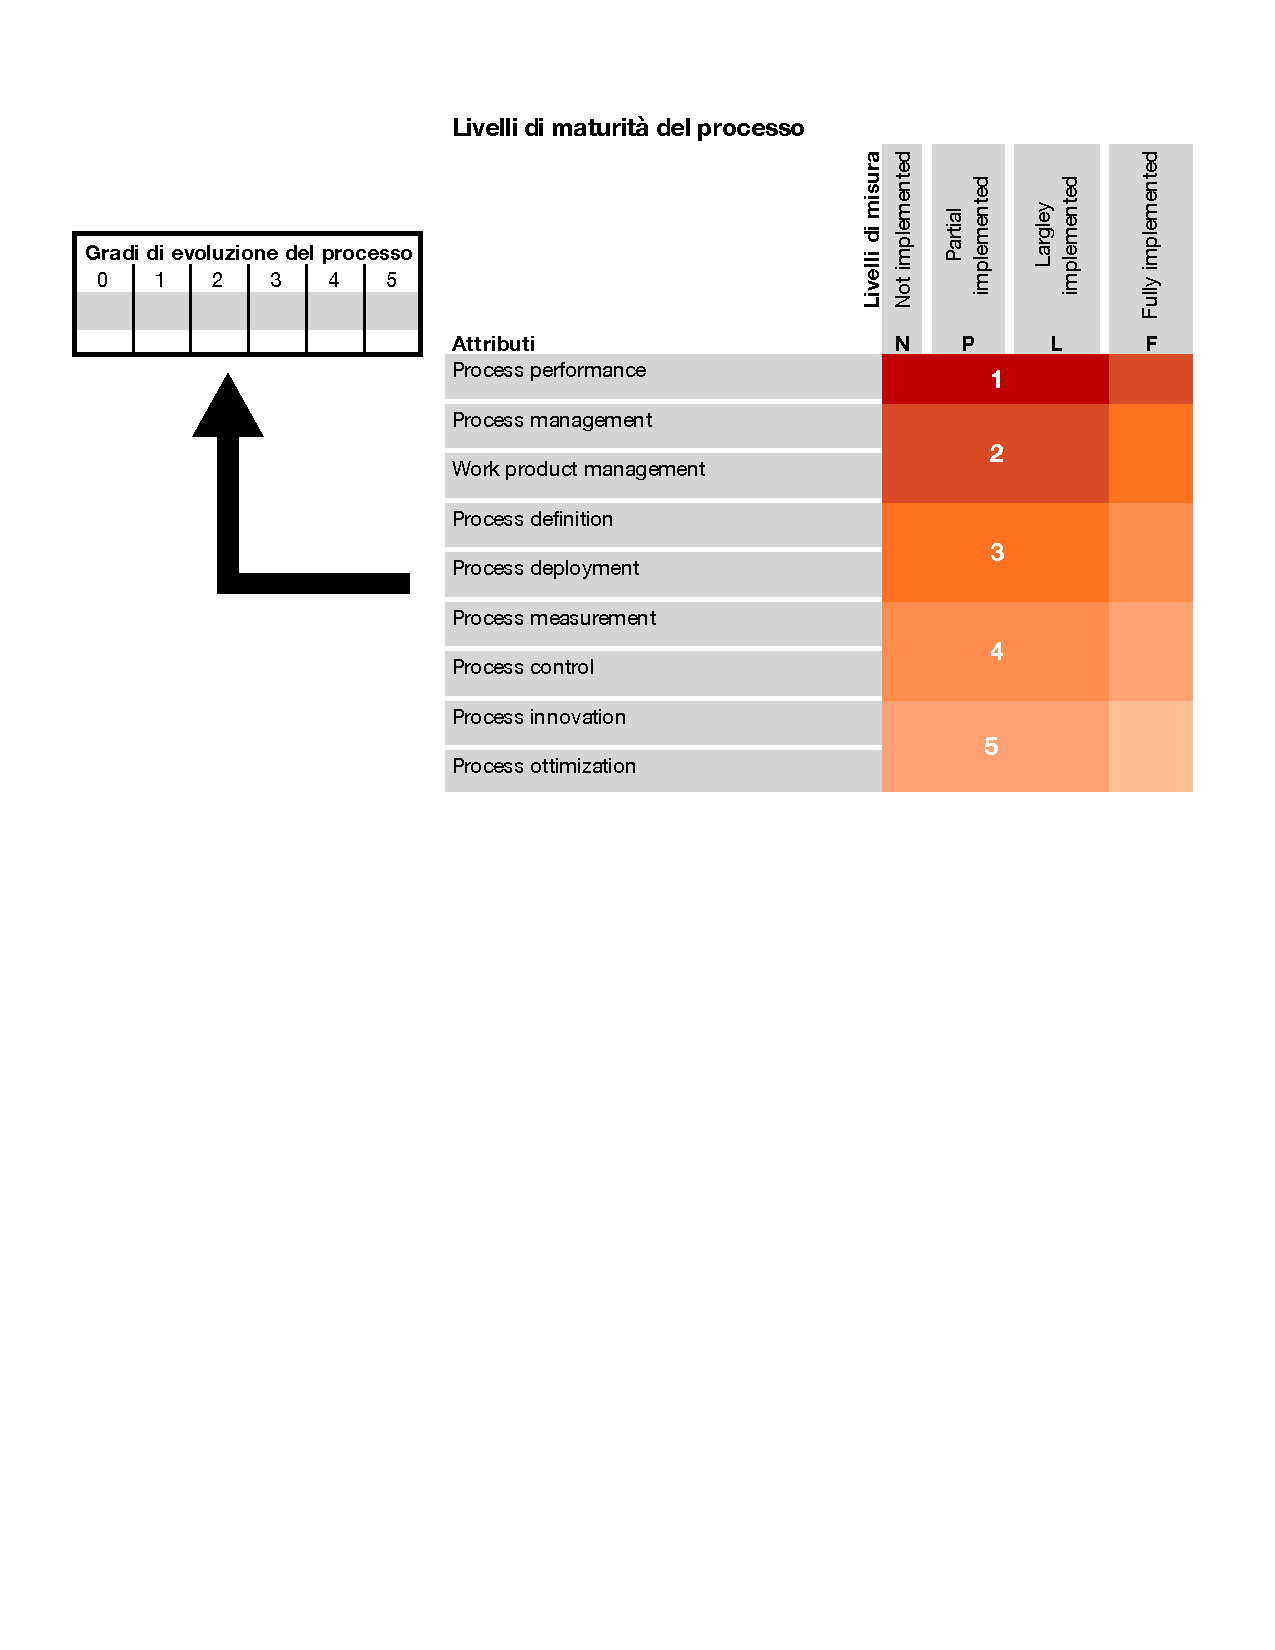
\includegraphics[scale=0.7]{images/ISOIEC15504.pdf}
	\caption{Riepilogo modello ISO/IEC 15504}
\end{figure}
\newpage

\subsection{Ciclo di Deming}
Il ciclo di Deming, noto anche come PDCA (dall'inglese \textbf{P}lan-\textbf{D}o-\textbf{C}heck-\textbf{A}ct), è un metodo di gestione iterativo suddiviso in quattro stadi ed utilizzato per il controllo del miglioramento continuo dei processi e dei prodotti. Esso permette, nello specifico, di migliorare gradualmente la qualità dei processi in termini di efficienza ed efficacia, ottimizzando l'uso delle risorse e misurando la loro conformità rispetto le aspettative. \\
La seguente immagine riporta le attività previste a tale scopo e ne segue una breve descrizione. 
\begin{figure}[htbp]
	\centering
	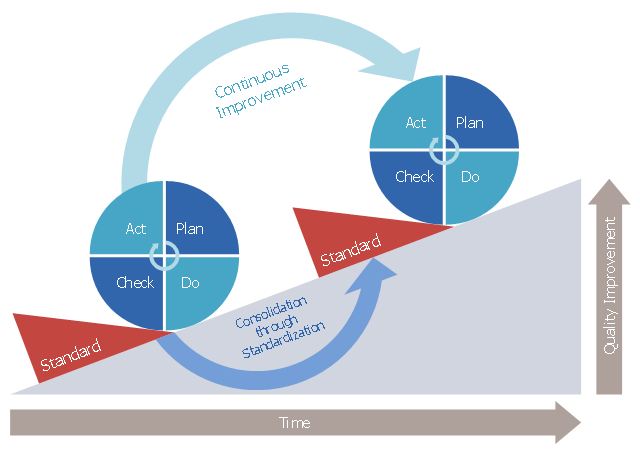
\includegraphics[scale=0.5]{images/pdca.png}
	\caption{Principio del miglioramento continuo secondo PDCA}
	
\end{figure}

\begin{itemize}
	\item \textbf{Plan}: prevede la definizione delle attività, scadenze, responsabilità e risorse atti a raggiungere e soddisfare degli obiettivi di miglioramento;
	\item \textbf{Do}: prevede l'esecuzione delle attività pianificate durante il periodo di pianificazione;
	\item \textbf{Check}: prevede la verifica dell'esito del processo in seguito all'attuazione delle strategie di miglioramento ed il confronto tra i risultati raccolti durante la fase Do e quelli attesi (specificati nella fase Plan) per stimare l'impatto effettivo del o dei miglioramenti apportati;
	\item \textbf{Act}: prevede l'attuazione delle strategie che hanno portato a dei miglioramenti. Nel caso i risultati attuali si distacchino da quelli previsti, si possono compiere delle azioni di correzione in seguito ad un'approfondita analisi delle cause di tale errore. 
\end{itemize}

\newpage
\section{ISO/IEC 9126}
Lo standard ISO/IEC 9126 definisce un modello dei requisiti qualitativi del Prodotto.
Il modello descritto si concentra in primo luogo sui tre punti di vista della qualità che esistono sul prodotto:
\begin{itemize}
	\item \textbf{Qualità esterna:} esprime il comportamento dinamico del software, in un determinato ambiente d'uso. In sostanza consiste nelle prestazioni e nelle funzionalità che il prodotto offre quando è in esecuzione;
	\item \textbf{Qualità interna:} esprime le proprietà statiche, cioè
	indipendenti dal contesto di esecuzione e uso. Sono direttamente misurabili ad esempio sul
	codice sorgente, pertanto senza la necessità di eseguire il software;
	\item \textbf{Qualità in uso:} esprime il livello con cui il prodotto si dimostra utile all'utente nel suo contesto d'uso. In altre parole rappresenta la capacità del prodotto di dare efficacia ed efficienza al lavoro dell'utente, a fronte di una sicurezza di utilizzo e di una soddisfazione nel far uso del prodotto.
\end{itemize}
\subsection{Modello per la qualità esterna ed interna}
Per la qualità esterna ed interna è definito un modello gerarchico formato da 6 caratteristiche principali e numerose sottocaratteristiche, tutte misurabili direttamente o indirettamente grazie all'utilizzo di metriche.
Le sei caratteristiche principali sono elencate di seguito:
\begin{itemize}
	\item \textbf{Funzionalità:} rappresenta la capacità del prodotto software di fornire funzioni che soddisfano le esigenze stabilite, sia esplicite che implicite, quando il software opera in un determinato contesto di utilizzo. Sottocaratteristiche notevoli sono l'interoperabilità e la Sicurezza, intesa come la capacità di proteggere le informazioni e i dati da accessi non autorizzati;
	\item \textbf{Affidabilità:} capacità di mantenere uno specificato livello di prestazione quando si opera in specificate condizioni. Sottocaratteristiche importanti sono la maturità e la tolleranza all'errore;
	\item \textbf{Efficienza:} capacità di fornire le funzioni richieste nel minor tempo possibile, sfruttando al meglio le risorse messe a disposizione;
	\item \textbf{Usabilità:} capacità del prodotto software di essere capito, appreso, usato e gradito all'utente, quando usato in contesti specificati. Una sottocaratteristica di rilievo è l'attrattiva;
	\item \textbf{Manutenibilità:} capacità del software di essere modificato e manutenuto. Per modifiche si intendono correzioni o adattamenti del software, negli ambienti, nei requisiti e nelle specifiche funzionali. Una sottocaratteristica importante è la testabilità, cioè la capacità di un software di consentire la verifica e di essere oggetto di test;
	\item \textbf{Portabilità:} capacità di poter essere trasferito da un ambiente di esecuzione all'altro.
\end{itemize}
\subsection{Modello per la qualità in uso}
Per la qualità in uso lo standard definisce una gerarchia separata, per enfatizzare il fatto che qui si considera non solo il prodotto software in sè, ma la relazione stretta tra esso e l'utente, nell'ambiente di utilizzo. Il modello è formato dalle seguenti quattro caratteristiche:
\begin{itemize}
	\item \textbf{Efficacia:} rappresenta la capacità di supportare un utente nel raggiungere i suoi obiettivi con accuratezza e completezza in un dato contesto;
	\item \textbf{Produttività:} la capacità di supportare un utente nello spendere l’appropriata quantità di risorse in relazione all’efficacia dei risultati da raggiungere; 
	\item \textbf{Soddisfazione:} la capacità di soddisfare un utente in un dato contesto d’uso;
	\item \textbf{Safety:} la capacità di raggiungere accettabili livelli di rischio di
	danni a persone, al software, ad apparecchiature, o all’ambiente operativo in un dato contesto d’uso.
\end{itemize}
\begin{figure}[htbp]
	\centering
	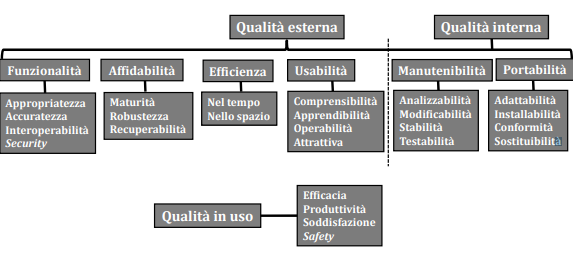
\includegraphics{images/gerarchiaQualitaProdotto.png}
	\caption{Riepilogo modello ISO 9126}
\end{figure}